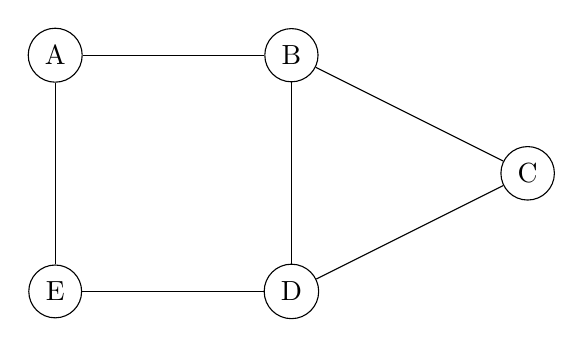
\begin{tikzpicture}
\node at (0,0) [draw,shape = circle](E){E};
\node at (3,0) [draw,shape = circle](D){D};
\node at (0,3) [draw,shape = circle](A){A};
\node at (3,3) [draw,shape = circle](B){B};
\node at (6,1.5) [draw,shape = circle](C){C};
\draw (A) -- (B);
\draw (B) -- (C);
\draw (C) -- (D);
\draw (D) -- (E);
\draw (A) -- (E);
\draw (B) -- (D);
\end{tikzpicture}